\documentclass[a4paper,titlepage]{article}

\usepackage{caption}
\usepackage{subcaption}
\usepackage{graphicx}
\usepackage[utf8]{inputenc}
\usepackage[italian]{babel}
\usepackage{csquotes}
\usepackage[T1]{fontenc}
\pdfsuppresswarningpagegroup=1
\graphicspath{ {images/} }

\title{Relazione del Progetto Laboratorio di ASD\\[0.5em]
\large Seconda Parte}
\date{Agosto 2021}
\author{
M. Giunta\thanks{Marco Giunta 147852 giunta.marco@spes.uniud.it} \and
S. Anzolin\thanks{Samuele Anzolin 142766  anzolin.samuele@spes.uniud.it} \and
F. Casani\thanks{Federico Casani 141212  casani.federico@spes.uniud.it} \and
G. De Nardi \thanks{Gianluca Giuseppe Maria De Nardi 142733 142733@spes.uniud.it}
}
% Disable indentation
\setlength{\parindent}{0pt}

\begin{document}
% Generate title page
\maketitle

% Generate TOC
\pagenumbering{arabic}
\tableofcontents
\newpage

\section{Introduzione}
In questo progetto analizzeremo i tempi di esecuzione per le operazioni di inserimento e ricerca sui tre principali alberi binari:
\begin{itemize}
  \item Red-Black Tree (\textbf{RBT})
  \item Adelson-Velsky and Landis Tree (\textbf{AVL})
  \item Binary Search Tree (\textbf{BST})
\end{itemize}
Utilizzeremo il linguaggio di programmazione \textbf{C} per la realizzazione del codice essendo un linguaggio veloce ed efficiente, ottenendo così dei tempi di esecuzione più puliti e liberi da azioni superflue.
\newpage

\section{Cenni Teorici}
Come accennato nel capitolo precedente andremo ad analizzare tre strutture dati, che seppur molto simili concettualmente, strutturalmente hanno delle differenze, andiamo ad analizzare queste strutture.

\subsection{BST, Binary search Tree}
I \textbf{Binary Search Tree} sono i più semplici sia dal punto di vista teorico, sia per quanto riguarda quello implementativo.
La regola fondamentale per la realizzazione di un BST è la seguente:

\begin{displayquote}
Per ogni nodo \(x \in T\) tutte le chiavi che si trovano nel sottoalbero radicato a sinistra del nodo x sono minori della chiave di x e tutte le chiavi che si trovano nel sottoalbero destro di x sono maggiori della chiave di x.
\end{displayquote}

Le operazioni che andremo ad analizzare hanno costo asintotico \(\Theta(n)\) nel caso peggiore,  nel caso medio \(\mathcal{O}(\log{}n)\) in entrambe le operazioni (inserimento e ricerca di un elemento).

\subsection{RBT, Red-Black Tree}
I \textbf{Red-Black Tree} sono una struttura ad albero derivata dai BST classici, dove ogni nodo ha un valore aggiuntivo \textit{colore}, che prenderà appunto valore o rosso, o nero, e servirà a mantere un’altezza dell’albero bilanciata da entrambi i lati.
La regola fondamentale dei RBT, oltre a quella derivata dai BST sarà:

\begin{displayquote}
L'altezza nera del sottoalbero radicato in un nodo X è definita come il massimo numero di nodi neri lungo un possibile cammino da x a una foglia, quindi per ogni nodo \(x \in T\), le altezze nere dei sotto-alberi di sinistra e di destra nel nodo x coincidono.
\end{displayquote}

Il loro costo asintotico è  \(\mathcal{O}(\log{}n)\) in qualsiasi caso.

\subsection{AVL, Adelson-Velsky and Landis Tree}

Gli \textbf{Adelson-Velsky and Landis Tree} sono anch’essi derivati dai classici BST e quindi mantengono la loro regola fondamentale, aggiungendo tuttavia un’altra regola:

\begin{displayquote}
Per ogni nodo  \(x \in T\) le altezze dei sotto-alberi radicati a sinistra e a destra del nodo x, differiscono al più di 1.
\end{displayquote}

Il costo asintotico delle operazioni sarà quindi, come per i RBT, \(\mathcal{O}(\log{}n)\) in tutti i casi. 
\newpage

\section{Aspettative}
Data la maggiore semplicità strutturale e il maggior costo asintotico dei Binary Search Tree ci aspetteremo una maggior inefficienza, che andrà peggiorando se l’albero si sbilancia.
Avremo quindi un albero più sbilanciato se l’input che andremo ad inserire è abbastanza ordinato.


I RBT e gli AVL hanno, invece, tempo asintotico logaritmico per qualsiasi tipo di input; tuttavia, gli AVL grazie alla loro \textquote{regola fondamentale} tendono a sbilanciarsi molto meno (al più di 1) rispetto ai RBT e quindi saranno teoricamente più efficienti nell’operazione di ricerca.
Nell’operazione di inserimento, i RBT effettuano al più due cammini radice-foglia, riducendosi a uno nel caso l’albero non sia da ribilanciare, mentre gli alberi AVL utilizzano sempre due cammini, uno per inserire l’elemento e uno per ribilanciare sempre l’albero, ci aspetteremo quindi un tempo di esecuzione più lungo per questi ultimi quando parliamo di operazioni di inserimento. 

\section{Implementazione}
Analizziamo adesso alcune note implementative che abbiamo riscontrato nella realizzazione del progetto, come l’impossibilità di utilizzare la deviazione standard come metodo di confronto, essa infatti ha un range troppo alto per essere utilizzata e abbiamo quindi ripiegato sull’utilizzo della mediana al posto della media, e della deviazione mediana assoluta (MAD) definita come:

\[MAD = (|X_i - median(X)|\]

Questi indici essendo più stabili e robusti ci hanno permesso di ottenere dati meno sensibili e quindi più precisi per le nostre misurazioni.
Per il calcolo della mediana abbiamo inoltre scelto di utilizzare \textit{Quicksort} come algoritmo per l’ordinamento del array, da cui poi estrapoliamo la mediana, essendo un algoritmo efficiente per l’utilizzo che ne facciamo. 

Andremo quindi ad analizzare i tempi medi ammortizzati per l’esecuzione di  operazioni di ricerca e inserimento delle tre tipologie di alberi, con il variare di \textit{n} tra 1000 e 1000000.
Il tempo ammortizzato per l’esecuzione viene calcolato nel seguente modo: 

\[Tempo Ammortizzato = \frac{tempoTotale}{n}\]

Il tempo ammortizzato non dovrà superare l’errore relativo del 1\%.
Da notare anche l’implementazione di un numero minimo di cicli (nel nostro caso 10) che andremo ad effettuare anche se l’errore assoluto è già stato superato.
\newpage

\section{Analisi dei dati ottenuti}

\subsection{Grafico dei tempi di esecuzione dei BST}

\begin{figure}[h]
  \centering
  \begin{subfigure}{\textwidth}
     \captionsetup{justification=centering}
     \caption{Deviazione Mediana Assoluta}
     \makebox[\textwidth][c]{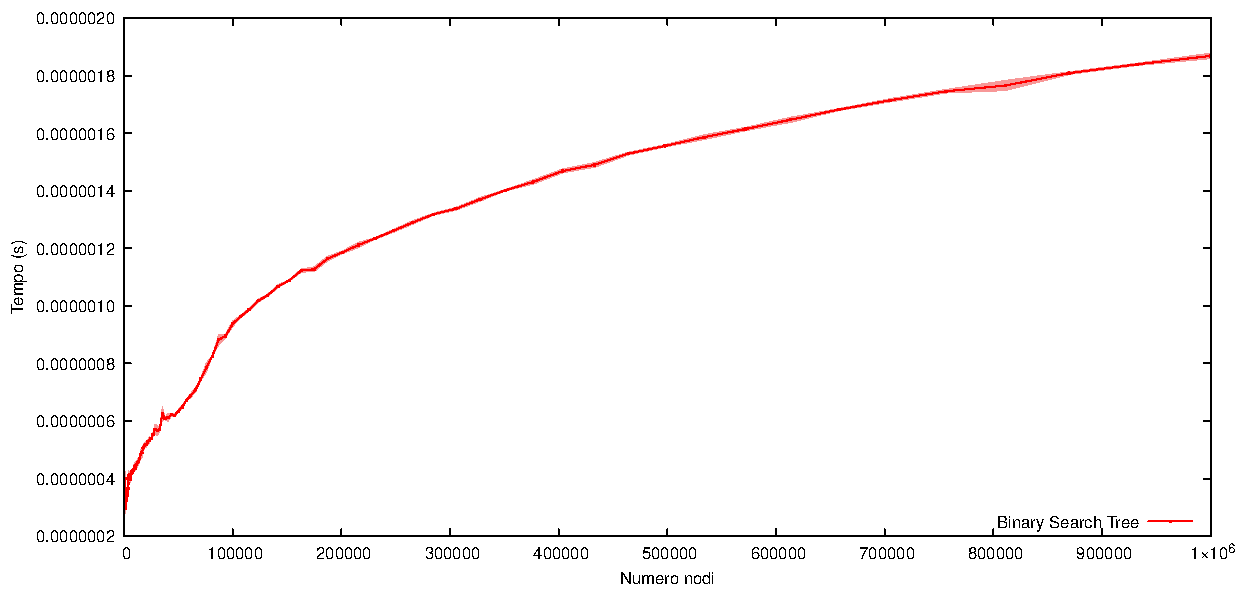
\includegraphics[width=1.24\textwidth]{bst_mad}}%
     \label{fig:bst_mad}
  \end{subfigure}%
  \vspace{2pt}
  \begin{subfigure}{\textwidth}
     \captionsetup{justification=centering}
     \caption{Confronto media/mediana}
     \makebox[\textwidth][c]{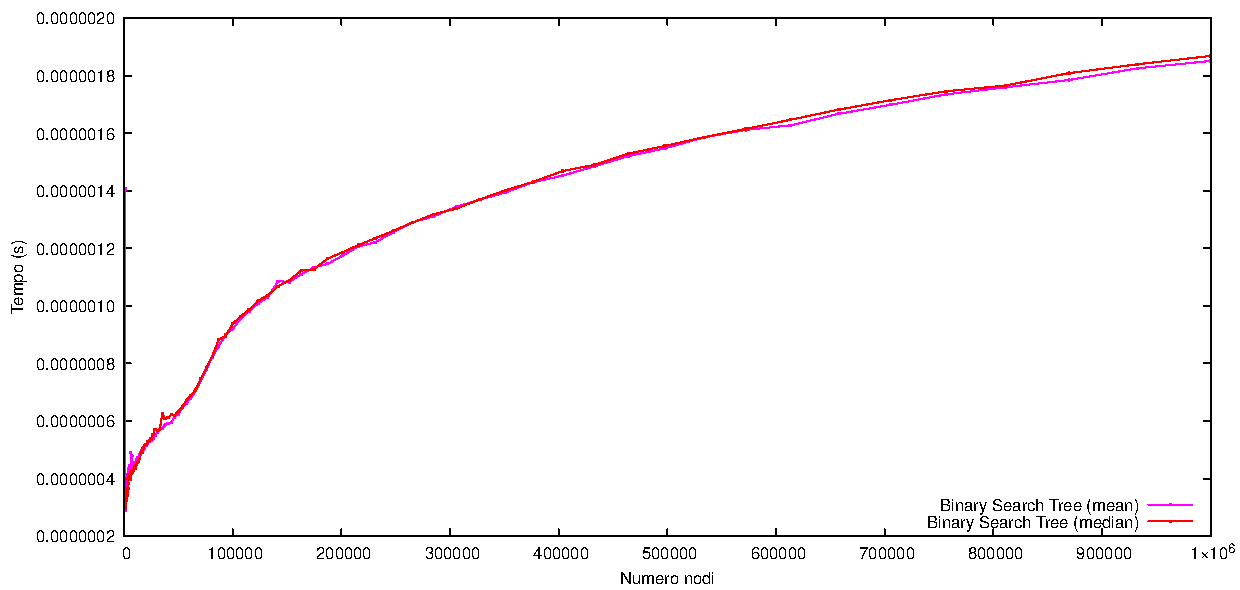
\includegraphics[width=1.24\textwidth]{bst_mean_median}}%
     \label{fig:bst_mean_median}
  \end{subfigure}
  \caption{Tempi di esecuzione con un BST}
\end{figure}
\newpage

\subsection{Grafici dei tempi di esecuzione dei RBT }

\begin{figure}[h]
  \centering
  \begin{subfigure}{\textwidth}
    \captionsetup{justification=centering}
    \caption{Deviazione Mediana Assoluta}
     \makebox[\textwidth][c]{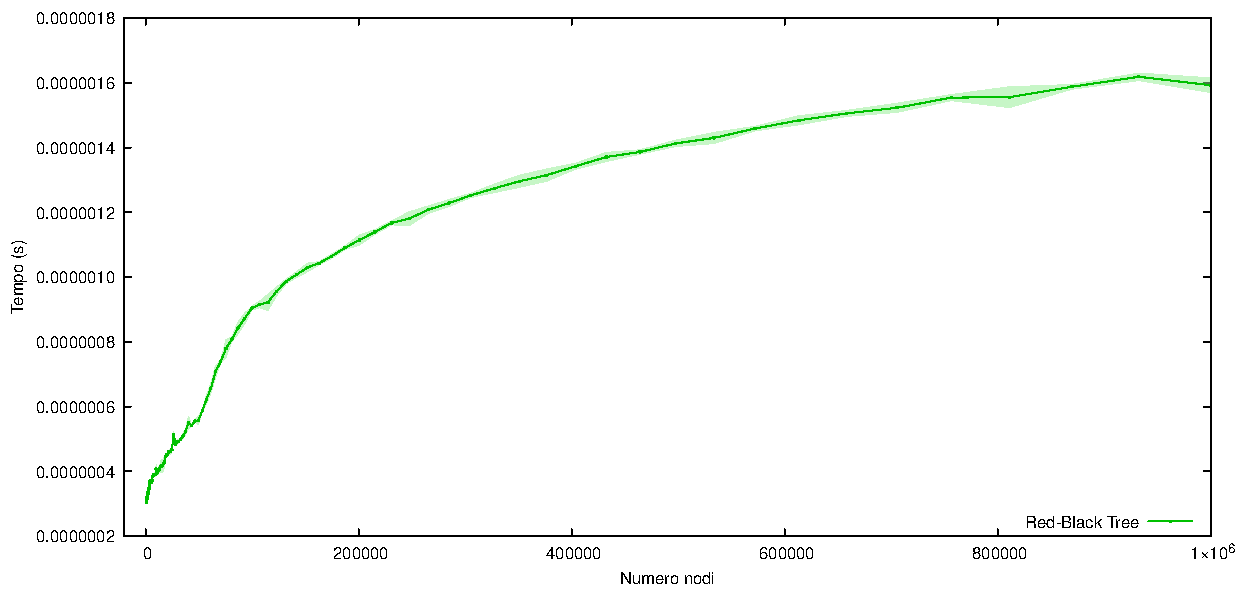
\includegraphics[width=1.24\textwidth]{rbt_mad}}%
     \label{fig:rbt_mad}
  \end{subfigure}%
   \vspace{2pt}
  \begin{subfigure}{\textwidth}
    \captionsetup{justification=centering}
     \caption{Confronto media/mediana}
     \makebox[\textwidth][c]{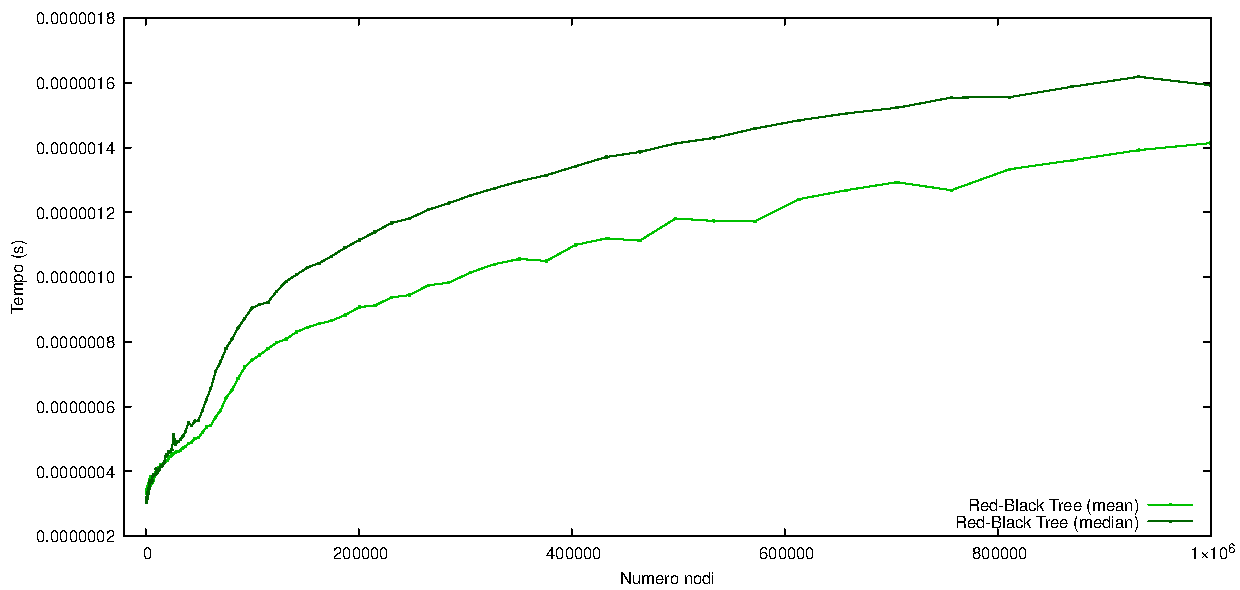
\includegraphics[width=1.24\textwidth]{rbt_mean_median}}%
     \label{fig:rbt_mean_median}
  \end{subfigure}
  \caption{Tempi di esecuzione con un RBT}
\end{figure}
\newpage

\subsection{Grafici dei tempi di esecuzione degli AVL }

\begin{figure}[h]
  \centering
  \begin{subfigure}{\textwidth}
    \captionsetup{justification=centering}
     \caption{Deviazione Mediana Assoluta}
     \makebox[\textwidth][c]{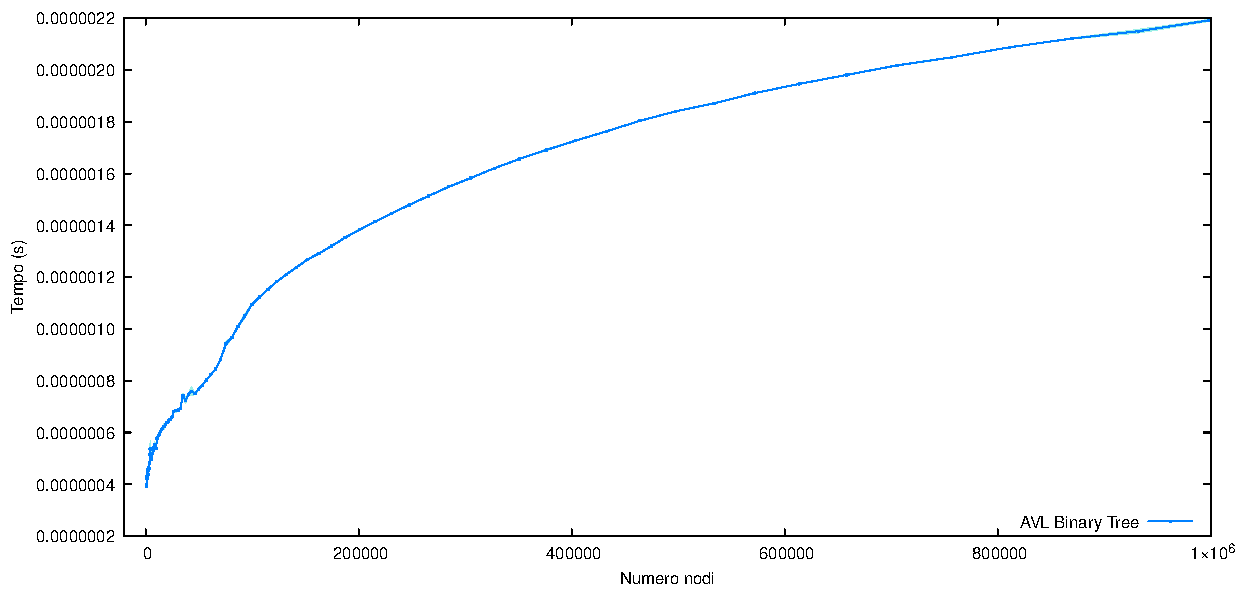
\includegraphics[width=1.2\textwidth]{avl_mad}}%
     \label{fig:avl_mad}
  \end{subfigure}%
  \vspace{2pt}
  \begin{subfigure}{\textwidth}
    \captionsetup{justification=centering}
     \caption{Confronto media/mediana}
     \makebox[\textwidth][c]{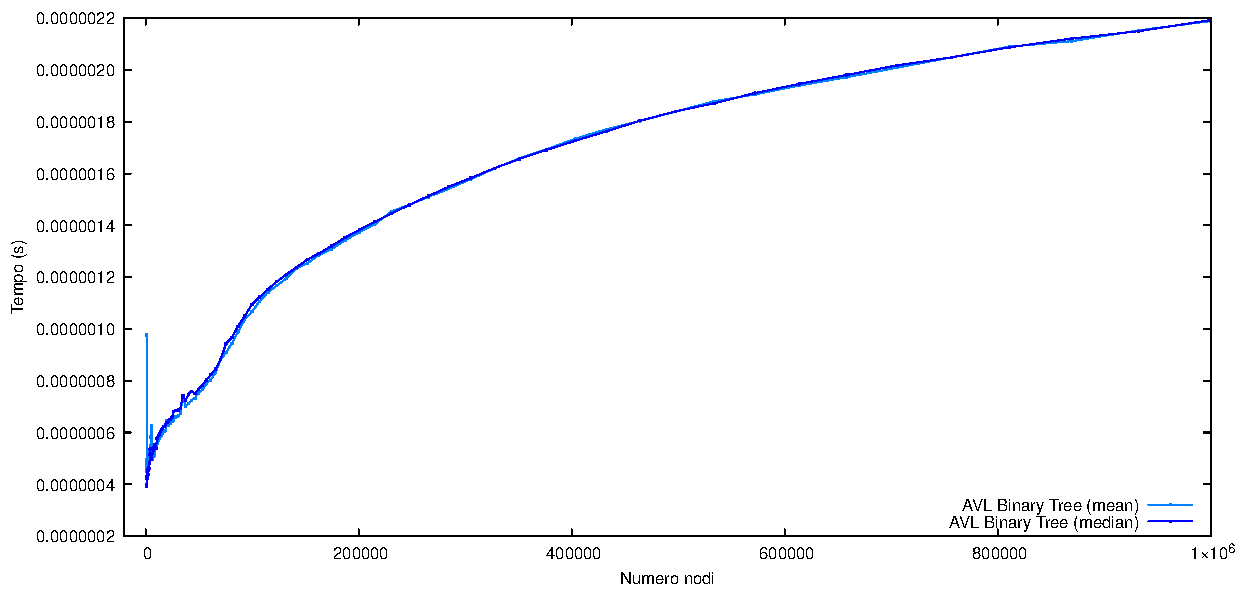
\includegraphics[width=1.2\textwidth]{avl_mean_median}}%
     \label{fig:avl_mean_median}
  \end{subfigure}
  \caption{Tempi di esecuzione con un AVL}
\end{figure}
\newpage

\subsection{Analisi comparativa tra i 3 alberi}

\begin{figure}[h]
  \centering
  \begin{subfigure}{\textwidth}
    \captionsetup{justification=centering}
     \caption{Deviazione Mediana Assoluta}
     \makebox[\textwidth][c]{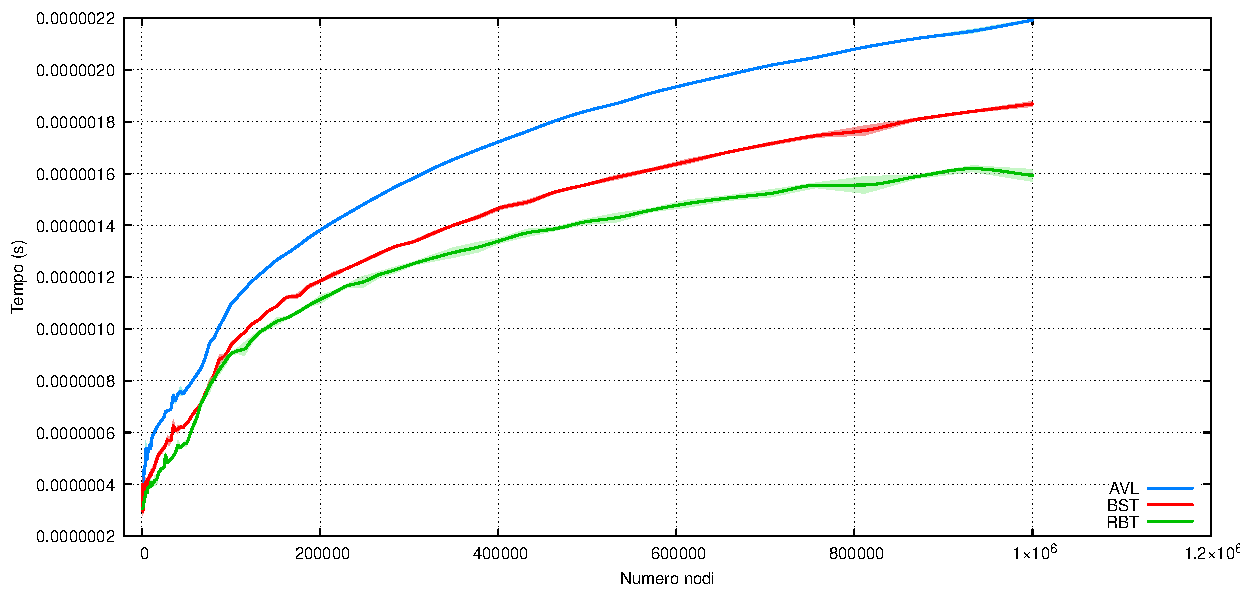
\includegraphics[width=1.2\textwidth]{bst_avl_rbt_median}}%
     \label{fig:bst_avl_rbt_median}
  \end{subfigure}%
  \vspace{2pt}
  \begin{subfigure}{\textwidth}
    \captionsetup{justification=centering}
    \caption{Confronto media/mediana}
     \makebox[\textwidth][c]{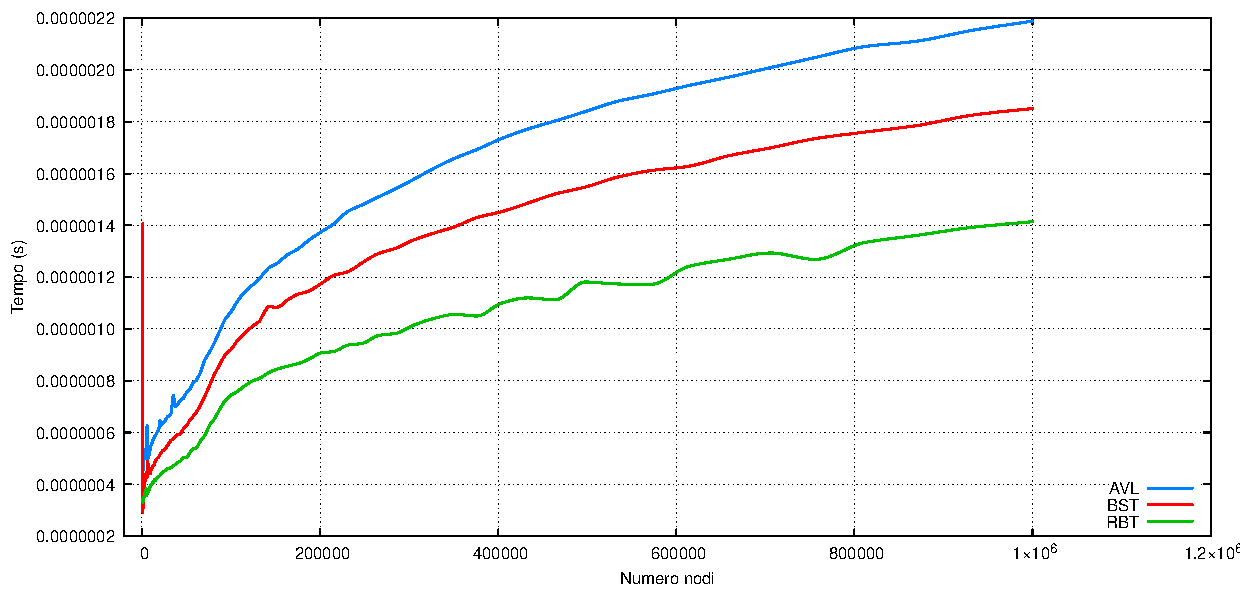
\includegraphics[width=1.2\textwidth]{bst_avl_rbt_mean}}%
     \label{fig:bst_avl_rbt_mean}
  \end{subfigure}
  \caption{Confronto tempi di esecuzione tra i 3 tipi di alberi}
\end{figure}

Come possiamo osservare dai grafici qui sopra riportati, la tipologia di albero più efficiente sono i \textbf{Red-Black Tree}, fermo restando che gli inserimenti sono casuali e che in altri contesti possiamo ottenere altri dati. Inaspettatamente i BST sono più efficienti dei rivali AVL forse per i numerosi cammini che effettuano gli alberi AVL per ribilanciare il tutto o forse per il fatto che gli inserimenti erano completamente casuali e quindi i BST non si sono sbilanciati più di tanto.
\newpage

\section{Conclusioni}

Come osservato da questa relazione, i \textbf{Red-Black Tree} si sono rivelati gli alberi più efficienti per l’inserimento e la ricerca di valori completamente casuali. Possiamo, infine affermare che questi studi sono molto importanti per la scelta di un albero binario, se il nostro scopo è avere un programma efficiente in termini di tempo.
\end{document}
